\begin{figure}[h!]
\captionsetup[subfigure]{justification=centering}
\centerline{
\subfloat[\(D2Q5\)]{\label{fig:D2Q5}
\centering
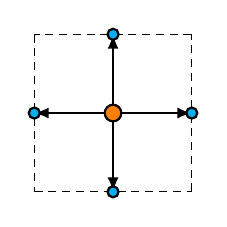
\begin{tikzpicture}[>=latex]
    \draw[densely dashed] (0,0) -- (2,0);
    \draw[densely dashed] (2,0) -- (2,2);
    \draw[densely dashed] (2,2) -- (0,2);
    \draw[densely dashed] (0,2) -- (0,0);
    \draw[ ->, thick] (1,1) -- (0,1);
    \draw[ ->, thick] (1,1) -- (1,0);
    \draw[ ->, thick] (1,1) -- (2,1);
    \draw[ ->, thick] (1,1) -- (1,2);
    \draw[thick,fill=orange](1,1) circle(3pt);
    \draw[thick,fill=cyan](0,1) circle(2pt);
    \draw[thick,fill=cyan](1,0) circle(2pt);
    \draw[thick,fill=cyan](2,1) circle(2pt);
    \draw[thick,fill=cyan](1,2) circle(2pt);
\end{tikzpicture}\hspace{1em}
}
\subfloat[\(D3Q7\)]{\label{fig:D3Q7}
\centering
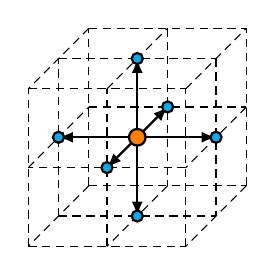
\begin{tikzpicture}[>=latex]
    \draw[densely dashed] (-2,0,0) -- (0,0,0);
    \draw[densely dashed] (-2,0,0) -- (-2,2,0);
    \draw[densely dashed] (-2,0,0) -- (-2,0,2);
    \draw[densely dashed] (-2,0,2) -- (0,0,2);
    \draw[densely dashed] (-2,2,0) -- (0,2,0);
    \draw[densely dashed] (-2,0,2) -- (-2,2,2);
    \draw[densely dashed] (-2,2,0) -- (-2,2,2);
    \draw[densely dashed] (-2,2,2) -- (0,2,2);
    \draw[densely dashed] (0,0,0) -- (0,0,2);
    \draw[densely dashed] (0,0,0) -- (0,2,0);
    \draw[densely dashed] (0,0,2) -- (0,2,2);
    \draw[densely dashed] (0,2,2) -- (0,2,0);
 	\draw[densely dashed] (-2,0,1) -- (0,0,1); 
	\draw[densely dashed] (-2,0,1) -- (-2,2,1); 
	\draw[densely dashed] (-2,2,1) -- (0,2,1); 
	\draw[densely dashed] (0,2,1) -- (0,0,1); 
	\draw[densely dashed] (-1,0,0) -- (-1,0,2); 
	\draw[densely dashed] (-1,0,2) -- (-1,2,2); 
	\draw[densely dashed] (-1,2,2) -- (-1,2,0); 
	\draw[densely dashed] (-1,2,0) -- (-1,0,0); 
	\draw[densely dashed] (-2,1,0) -- (0,1,0); 
	\draw[densely dashed] (0,1,0) -- (0,1,2); 
	\draw[densely dashed] (0,1,2) -- (-2,1,2); 
	\draw[densely dashed] (-2,1,2) -- (-2,1,0); 
	\draw[->,thick](-1,1,1) -- (-1,1,0);
    \draw[->,thick](-1,1,1) -- (-1,2,1);
    \draw[->,thick](-1,1,1) -- (-1,1,2);
    \draw[->,thick](-1,1,1) -- (0,1,1);
    \draw[->,thick](-1,1,1) -- (-2,1,1);
    \draw[->,thick](-1,1,1) -- (-1,0,1);
    \draw[thick,fill=orange](-1,1,1) circle(3pt);
	\draw[thick,fill=cyan](-1,1,0) circle(2pt);     
	\draw[thick,fill=cyan](-1,2,1) circle(2pt);
    \draw[thick,fill=cyan](-1,1,2) circle(2pt);
    \draw[thick,fill=cyan](0,1,1) circle(2pt);
    \draw[thick,fill=cyan](-2,1,1) circle(2pt);
    \draw[thick,fill=cyan](-1,0,1) circle(2pt);
\end{tikzpicture}\hspace{1em}
}
\subfloat[\(D2Q9\)]{\label{fig:D2Q9}
\centering
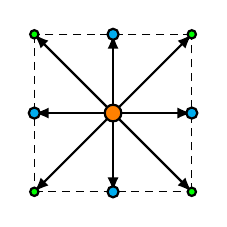
\begin{tikzpicture}[>=latex]
    \draw[densely dashed] (0,0) -- (2,0);
    \draw[densely dashed] (2,0) -- (2,2);
    \draw[densely dashed] (2,2) -- (0,2);
    \draw[densely dashed] (0,2) -- (0,0);
    \draw[ ->, thick] (1,1) -- (0,1);
    \draw[ ->, thick] (1,1) -- (1,0);
    \draw[ ->, thick] (1,1) -- (2,1);
    \draw[ ->, thick] (1,1) -- (1,2);
    \draw[ ->, thick] (1,1) -- (2,2);
    \draw[ ->, thick] (1,1) -- (0,2);
    \draw[ ->, thick] (1,1) -- (0,0);
    \draw[ ->, thick] (1,1) -- (2,0);
    \draw[thick,fill=orange](1,1) circle(3pt);
    \draw[thick,fill=cyan](0,1) circle(2pt);
    \draw[thick,fill=cyan](1,0) circle(2pt);
    \draw[thick,fill=cyan](2,1) circle(2pt);
    \draw[thick,fill=cyan](1,2) circle(2pt);
    \draw[thick,fill=green](2,2) circle(1.5pt);
    \draw[thick,fill=green](0,2) circle(1.5pt);
    \draw[thick,fill=green](0,0) circle(1.5pt);
    \draw[thick,fill=green](2,0) circle(1.5pt);
\end{tikzpicture}\hspace{1em}
}
\subfloat[\(D3Q19\)]{\label{fig:D3Q19}
\centering
 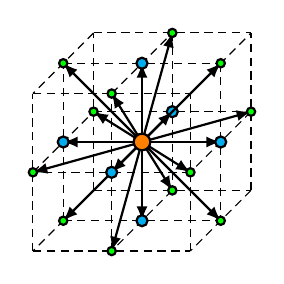
\begin{tikzpicture}[>=latex]
 	% dashing
    \draw[densely dashed] (-2,0,0) -- (0,0,0);
    \draw[densely dashed] (-2,0,0) -- (-2,2,0);
    \draw[densely dashed] (-2,0,0) -- (-2,0,2);
    \draw[densely dashed] (-2,0,2) -- (0,0,2);
    \draw[densely dashed] (-2,2,0) -- (0,2,0);
    \draw[densely dashed] (-2,0,2) -- (-2,2,2);
    \draw[densely dashed] (-2,2,0) -- (-2,2,2);
    \draw[densely dashed] (-2,2,2) -- (0,2,2);
    \draw[densely dashed] (0,0,0) -- (0,0,2);
    \draw[densely dashed] (0,0,0) -- (0,2,0);
    \draw[densely dashed] (0,0,2) -- (0,2,2);
    \draw[densely dashed] (0,2,2) -- (0,2,0);
 	\draw[densely dashed] (-2,0,1) -- (0,0,1); 
	\draw[densely dashed] (-2,0,1) -- (-2,2,1); 
	\draw[densely dashed] (-2,2,1) -- (0,2,1); 
	\draw[densely dashed] (0,2,1) -- (0,0,1); 
	\draw[densely dashed] (-1,0,0) -- (-1,0,2); 
	\draw[densely dashed] (-1,0,2) -- (-1,2,2); 
	\draw[densely dashed] (-1,2,2) -- (-1,2,0); 
	\draw[densely dashed] (-1,2,0) -- (-1,0,0); 
	\draw[densely dashed] (-2,1,0) -- (0,1,0); 
	\draw[densely dashed] (0,1,0) -- (0,1,2); 
	\draw[densely dashed] (0,1,2) -- (-2,1,2); 
	\draw[densely dashed] (-2,1,2) -- (-2,1,0);   
	% back layer   
    \draw[->,thick](-1,1,1) -- (-1,1,0);
    \draw[->,thick](-1,1,1) -- (-2,1,0);
    \draw[->,thick](-1,1,1) -- (-1,2,0);
    \draw[->,thick](-1,1,1) -- (-1,0,0);
    \draw[->,thick](-1,1,1) -- (0,1,0);
    \draw[thick,fill=cyan](-1,1,0) circle(2pt);     
	\draw[thick,fill=green](-2,1,0) circle(1.5pt);
  	\draw[thick,fill=green](-1,2,0) circle(1.5pt);
  	\draw[thick,fill=green](-1,0,0) circle(1.5pt);
	\draw[thick,fill=green](0,1,0) circle(1.5pt);
  	% mid layer 
    \draw[->,thick](-1,1,1) -- (-1,2,1);
    \draw[->,thick](-1,1,1) -- (0,1,1);
    \draw[->,thick](-1,1,1) -- (-2,1,1);
    \draw[->,thick](-1,1,1) -- (-1,0,1);
    \draw[->,thick](-1,1,1) -- (-2,0,1);
    \draw[->,thick](-1,1,1) -- (0,0,1);
    \draw[->,thick](-1,1,1) -- (-2,2,1);
    \draw[->,thick](-1,1,1) -- (0,2,1);
	\draw[thick,fill=cyan](-1,2,1) circle(2pt);
    \draw[thick,fill=cyan](0,1,1) circle(2pt);
    \draw[thick,fill=cyan](-1,0,1) circle(2pt);
    \draw[thick,fill=cyan](-2,1,1) circle(2pt);
    \draw[thick,fill=green](-2,0,1) circle(1.5pt);     
  	\draw[thick,fill=green](0,0,1) circle(1.5pt);
    \draw[thick,fill=green](-2,2,1) circle(1.5pt);     
  	\draw[thick,fill=green](0,2,1) circle(1.5pt);
	% front layer 
	\draw[->,thick](-1,1,1) -- (-1,1,2);
    \draw[->,thick](-1,1,1) -- (-1,0,2);
	\draw[->,thick](-1,1,1) -- (-2,1,2);
	\draw[->,thick](-1,1,1) -- (0,1,2);
	\draw[->,thick](-1,1,1) -- (-1,2,2);
    \draw[thick,fill=cyan](-1,1,2) circle(2pt);
	\draw[thick,fill=green](-1,0,2) circle(1.5pt);
	\draw[thick,fill=green](-2,1,2) circle(1.5pt);
	\draw[thick,fill=green](0,1,2) circle(1.5pt);
	\draw[thick,fill=green](-1,2,2) circle(1.5pt);
	% origin
    \draw[thick,fill=orange](-1,1,1) circle(3pt);
  \end{tikzpicture}
}
\hspace{2em}
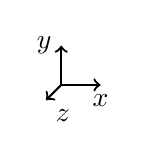
\begin{tikzpicture}
	\draw[->,thick] (0,0,0) -- (.5,0,0);
    \node[anchor=north] at (.5,0,0) {$x$};
    \draw[->,thick] (0,0,0) -- (0,.5,0);
    \node[anchor=east] at (0,.5,0) {$y$};
	\draw[->,thick] (0,0,0) -- (0,0,.5);
	\node[anchor=north west] at (0,0,.5) {$z$};
\end{tikzpicture}
}
\caption{Exemplary discrete velocity sets used for the descriptors implemented in \OpenLB. 
(a, b): \(DdQ(2d+1)\) for \(d=2,3\), respectively; (c): \(D2Q9\); (d): \(D3Q19\).  
Coloring refers to the corresponding energy shell, where orange, cyan and green denote zeroth, first and second order nodes, respectively. 
Figure reproduced from \cite{simonis:23b}.}
\label{fig:discreteVelocitySets}  
\end{figure}